\iffalse
\let\negmedspace\undefined
\let\negthickspace\undefined
\documentclass[journal,12pt,onecolumn]{IEEEtran}
\usepackage{cite}
\usepackage{amsmath,amssymb,amsfonts,amsthm}
\usepackage{algorithmic}
\usepackage{graphicx}
\usepackage{textcomp}
\usepackage{xcolor}
\usepackage{txfonts}
\usepackage{listings}
\usepackage{enumitem}
\usepackage{mathtools}
\usepackage{gensymb}
\usepackage[breaklinks=true]{hyperref}
\usepackage{tkz-euclide} % loads  TikZ and tkz-base
\usepackage{listings}



\newtheorem{theorem}{Theorem}[section]
\newtheorem{problem}{Problem}
\newtheorem{proposition}{Proposition}[section]
\newtheorem{lemma}{Lemma}[section]
\newtheorem{corollary}[theorem]{Corollary}
\newtheorem{example}{Example}[section]
\newtheorem{definition}[problem]{Definition}
%\newtheorem{thm}{Theorem}[section] 
%\newtheorem{defn}[thm]{Definition}
%\newtheorem{algorithm}{Algorithm}[section]
%\newtheorem{cor}{Corollary}
\newcommand{\BEQA}{\begin{eqnarray}}
\newcommand{\EEQA}{\end{eqnarray}}
\newcommand{\define}{\stackrel{\triangle}{=}}
\theoremstyle{remark}
\newtheorem{rem}{Remark}
%\bibliographystyle{ieeetr}
\begin{document}
%
\providecommand{\pr}[1]{\ensuremath{\Pr\left(#1\right)}}
\providecommand{\prt}[2]{\ensuremath{p_{#1}^{\left(#2\right)} }}        % own macro for this question
\providecommand{\qfunc}[1]{\ensuremath{Q\left(#1\right)}}
\providecommand{\sbrak}[1]{\ensuremath{{}\left[#1\right]}}
\providecommand{\lsbrak}[1]{\ensuremath{{}\left[#1\right.}}
\providecommand{\rsbrak}[1]{\ensuremath{{}\left.#1\right]}}
\providecommand{\brak}[1]{\ensuremath{\left(#1\right)}}
\providecommand{\lbrak}[1]{\ensuremath{\left(#1\right.}}
\providecommand{\rbrak}[1]{\ensuremath{\left.#1\right)}}
\providecommand{\cbrak}[1]{\ensuremath{\left\{#1\right\}}}
\providecommand{\lcbrak}[1]{\ensuremath{\left\{#1\right.}}
\providecommand{\rcbrak}[1]{\ensuremath{\left.#1\right\}}}
\newcommand{\sgn}{\mathop{\mathrm{sgn}}}
\providecommand{\abs}[1]{\left\vert#1\right\vert}
\providecommand{\res}[1]{\Res\displaylimits_{#1}} 
\providecommand{\norm}[1]{\left\lVert#1\right\rVert}
%\providecommand{\norm}[1]{\lVert#1\rVert}
\providecommand{\mtx}[1]{\mathbf{#1}}
\providecommand{\mean}[1]{E\left[ #1 \right]}
\providecommand{\cond}[2]{#1\middle|#2}
\providecommand{\fourier}{\overset{\mathcal{F}}{ \rightleftharpoons}}
\newenvironment{amatrix}[1]{%
  \left(\begin{array}{@{}*{#1}{c}|c@{}}
}{%
  \end{array}\right)
}
%\providecommand{\hilbert}{\overset{\mathcal{H}}{ \rightleftharpoons}}
%\providecommand{\system}{\overset{\mathcal{H}}{ \longleftrightarrow}}
	%\newcommand{\solution}[2]{\textbf{Solution:}{#1}}
\newcommand{\solution}{\noindent \textbf{Solution: }}
\newcommand{\cosec}{\,\text{cosec}\,}
\providecommand{\dec}[2]{\ensuremath{\overset{#1}{\underset{#2}{\gtrless}}}}
\newcommand{\myvec}[1]{\ensuremath{\begin{pmatrix}#1\end{pmatrix}}}
\newcommand{\mydet}[1]{\ensuremath{\begin{vmatrix}#1\end{vmatrix}}}
\newcommand{\myaugvec}[2]{\ensuremath{\begin{amatrix}{#1}#2\end{amatrix}}}
\providecommand{\rank}{\text{rank}}
\providecommand{\pr}[1]{\ensuremath{\Pr\left(#1\right)}}
\providecommand{\qfunc}[1]{\ensuremath{Q\left(#1\right)}}
	\newcommand*{\permcomb}[4][0mu]{{{}^{#3}\mkern#1#2_{#4}}}
\newcommand*{\perm}[1][-3mu]{\permcomb[#1]{P}}
\newcommand*{\comb}[1][-1mu]{\permcomb[#1]{C}}
\providecommand{\qfunc}[1]{\ensuremath{Q\left(#1\right)}}
\providecommand{\gauss}[2]{\mathcal{N}\ensuremath{\left(#1,#2\right)}}
\providecommand{\diff}[2]{\ensuremath{\frac{d{#1}}{d{#2}}}}
\providecommand{\myceil}[1]{\left \lceil #1 \right \rceil }
\newcommand\figref{Fig.~\ref}
\newcommand\tabref{Table~\ref}
\newcommand{\sinc}{\,\text{sinc}\,}
\newcommand{\rect}{\,\text{rect}\,}
%%
%	%\newcommand{\solution}[2]{\textbf{Solution:}{#1}}
%\newcommand{\solution}{\noindent \textbf{Solution: }}
%\newcommand{\cosec}{\,\text{cosec}\,}
%\numberwithin{equation}{section}
%\numberwithin{equation}{subsection}
%\numberwithin{problem}{section}
%\numberwithin{definition}{section}
%\makeatletter
%\@addtoreset{figure}{problem}
%\makeatother

%\let\StandardTheFigure\thefigure
\let\vec\mathbf

\bibliographystyle{IEEEtran}


\vspace{3cm}



\bigskip

\renewcommand{\thefigure}{\theenumi}
\renewcommand{\thetable}{\theenumi}
%\renewcommand{\theequation}{\theenumi}


Q. Find the equations of $AD$ , $BE$ and $CF$.
\fi
\\ \solution:
$\vec{D}$,$\vec{E}$,$\vec{F}$ are the midpoints of $BC$,$CA$,$AB$ respectively, then\\
\begin{align}
 \vec{D} &=  \myvec{\frac{-7}{2}\\\frac{1}{2}}\\
 \vec{E} &=  \myvec{-1\\-3}\\
 \vec{F} &= \myvec{\frac{-3}{2}\\\frac{5}{2}}
\end{align}
\begin{enumerate}
 \item The normal equation for the median $AD$ is
  \begin{align}
    \vec{n}^{\top}\myvec{\vec{x}-\vec{A}}&=0\\
    \implies
    \vec{n}^{\top}\vec{x}&=\vec{n}^{\top}\vec{A}
  \end{align}
 We have to find the $\vec{n}$ so that we can find $\vec{n}^{\top}$.
 Since,
\begin{align}
  \vec{n} &= \myvec{0 & 1\\
  -1 & 0}\vec{m}
\end{align}
Here $\vec{m} = \vec{D}- \vec{A}$ for median $AD$
\begin{align}
\vec{m}&=\myvec{\frac{-7}{2}\\\frac{1}{2}} - \myvec{1\\-1}\\
       &=\myvec{\frac{-9}{2}\\\frac{3}{2}}
\end{align}
Since,
\begin{align}
  \vec{n} &= \myvec{0 & 1\\
  -1 & 0}\vec{m}\\
\implies
\vec{n} &= \myvec{0 & 1\\
  -1 & 0}\myvec{\frac{-9}{2}\\\frac{3}{2}}\\
        &= \myvec{\frac{3}{2}\\\frac{9}{2}}
\end{align}
Hence the normal equation of median $AD$ is 
\begin{align}
    \myvec{\frac{3}{2} & \frac{9}{2}}\vec{x}&=\myvec{\frac{3}{2} & \frac{9}{2}}\myvec{1\\-1}\\
    \implies
    \myvec{\frac{3}{2} & \frac{9}{2}}\vec{x}&=-3
\end{align}
\item The normal equation for the median $BE$ is
\begin{align}
\vec{n}^{\top}\myvec{\vec{x}-\vec{B}}&=0\\
\implies
\vec{n}^{\top}\vec{x}&=\vec{n}^{\top}\vec{B}
\end{align}
Here $\vec{m} = \vec{E}- \vec{B}$ for median $BE$
\begin{align}
\vec{m}&=\myvec{-1\\-3} - \myvec{-4\\6}\\
       &=\myvec{3\\-9}
\end{align}
Since,
\begin{align}
  \vec{n} &= \myvec{0 & 1\\
  -1 & 0}\vec{m}\\
\implies
\vec{n} &= \myvec{0 & 1\\
  -1 & 0}\myvec{3\\-9}\\
        &= \myvec{-9\\-3}
\end{align}
Hence the normal equation of median $BE$ is 
\begin{align}
    \myvec{-9 & -3}\vec{x}&=\myvec{-9 & -3}\myvec{-4\\6}\\
\implies
    \myvec{-9 & -3}\vec{x}&=18
\end{align}
\item The normal equation for the median $CF$ is
\begin{align}
\vec{n}^{\top}\myvec{\vec{x}-\vec{C}}&=0\\
\implies
\vec{n}^{\top}\vec{x}&=\vec{n}^{\top}\vec{C}
\end{align}
Here $\vec{m} = \vec{F}- \vec{C}$ for median $CF$
\begin{align}
\vec{m}&=\myvec{\frac{-3}{2}\\\frac{5}{2}} - \myvec{-3\\-5}\\
       &=\myvec{\frac{3}{2}\\\frac{15}{2}}
\end{align}
Since,
\begin{align}
  \vec{n} &= \myvec{0 & 1\\
  -1 & 0}\vec{m}\\
\implies
\vec{n} &= \myvec{0 & 1\\
  -1 & 0}\myvec{\frac{3}{2}\\\frac{15}{2}}\\
        &= \myvec{\frac{15}{2}\\\frac{-3}{2}}
\end{align}
Hence the normal equation of median $CF$ is 
\begin{align}
    \myvec{\frac{15}{2} & \frac{-3}{2}}\vec{x}&=\myvec{\frac{15}{2} & \frac{-3}{2}}\myvec{-3\\-5}\\
\implies
    \myvec{\frac{15}{2} & \frac{-3}{2}}\vec{x}&=-15
\end{align}
\end{enumerate}
\begin{figure}
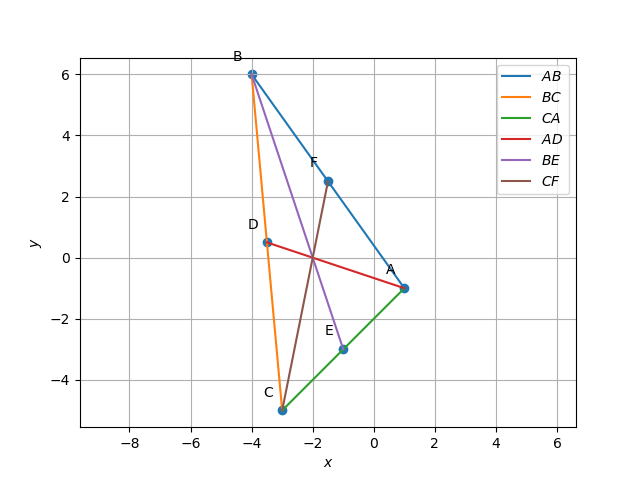
\includegraphics [width=\columnwidth] {./figs/figure.png}
\caption{ Medians $AD$ , $BE$ and $CF$}
\label{fig: medians}
\end{figure}



